% !TEX TS-program = pdflatex
% !TEX encoding = UTF-8 Unicode

% This is a simple template for a LaTeX document using the "article" class.
% See "book", "report", "letter" for other types of document.

\documentclass[11pt]{article} % use larger type; default would be 10pt

\usepackage[utf8]{inputenc} % set input encoding (not needed with XeLaTeX)

%%% Examples of Article customizations
% These packages are optional, depending whether you want the features they provide.
% See the LaTeX Companion or other references for full information.

%%% PAGE DIMENSIONS
\usepackage{geometry} % to change the page dimensions
\geometry{a4paper} % or letterpaper (US) or a5paper or....
% \geometry{margin=2in} % for example, change the margins to 2 inches all round
% \geometry{landscape} % set up the page for landscape
%   read geometry.pdf for detailed page layout information

\usepackage{graphicx} % support the \includegraphics command and options

% \usepackage[parfill]{parskip} % Activate to begin paragraphs with an empty line rather than an indent

%%% PACKAGES
\usepackage{booktabs} % for much better looking tables
\usepackage{array} % for better arrays (eg matrices) in maths
\usepackage{paralist} % very flexible & customisable lists (eg. enumerate/itemize, etc.)
\usepackage{verbatim} % adds environment for commenting out blocks of text & for better verbatim
\usepackage{subfig} % make it possible to include more than one captioned figure/table in a single float
% These packages are all incorporated in the memoir class to one degree or another...

%%% HEADERS & FOOTERS
\usepackage{fancyhdr} % This should be set AFTER setting up the page geometry
\pagestyle{fancy} % options: empty , plain , fancy
\renewcommand{\headrulewidth}{0pt} % customise the layout...
\lhead{}\chead{}\rhead{}
\lfoot{}\cfoot{\thepage}\rfoot{}

%%% SECTION TITLE APPEARANCE
\usepackage{sectsty}
\allsectionsfont{\sffamily\mdseries\upshape} % (See the fntguide.pdf for font help)
% (This matches ConTeXt defaults)

%%% ToC (table of contents) APPEARANCE
\usepackage[nottoc,notlof,notlot]{tocbibind} % Put the bibliography in the ToC
\usepackage[titles,subfigure]{tocloft} % Alter the style of the Table of Contents
\renewcommand{\cftsecfont}{\rmfamily\mdseries\upshape}
\renewcommand{\cftsecpagefont}{\rmfamily\mdseries\upshape} % No bold!

%%% END Article customizations

%%% The "real" document content comes below...

\title{Dossier de validation - IHM}
\author{Brahim Berkati}
%\date{} % Activate to display a given date or no date (if empty),
         % otherwise the current date is printed 

\begin{document}
\maketitle

\section{Introduction}
\paragraph{}
Ce document contient l'ensemble des informations concernant l'interface et la validation de cette dernière. Le document est divisé en quatres parties.
\paragraph{}
Dans un premier temps, nous explicitons certains concepts requis pour comprendre le fonctionnement technique de la LibGDX. Ensuite, nous justifierons les choix effectués pour améliorer l'ergonomie de l'application. La troisième partie couvre les procédures de validation utilisées en interne pour garantir la stabilité de l'interface. Enfin, nous terminons par décrire les méthodes de validations par des utilisateurs externes au projet.

\section{Structure de l'interface}
\paragraph{}
L'interface graphique est complètement géré par une librairie externe appelée LibGDX. Cette libraire affiche ce qu'on appelle un Screen qui contient toutes les informations de la scène. Un seul Screen est actif simultanément. C'est à travers l'utilisation de la méthode setScreen(Screen screen); que les changements sont effectués.
\paragraph{}
Sur une scène, il est possible d'afficher des sprites ainsi que divers widgets. Tous les widgets chargent une apparence en fonction de ce qu'on appelle un Skin. Le Skin contient toutes les informations en ce qui concerne l'ensemble des widgets. Cela permet d'uniformiser l'apparence de ces derniers.
\paragraph{}
L'ensemble des scènes comprennent donc un ensemble de widgets. Ces informations sont donc redondantes. Nous avons donc décidé de créer une abstraction d'une scène contenant toutes ces informations redondantes.

\section{Prototypage}
\paragraph{}
L'interface du jeu doit allié ergonomie et attractivité visuelle. Le meilleur moyen d'obtenir une ergonomie suffisante est de s'inspirer d'autres interfaces de jeux de plateau déjà existant. Ainsi, nous avons testé plusieurs jeux de Tablut en ligne, mais nous avons également recherché l'inspiration du côté des jeux d’échecs ainsi que du jeu "42 jeux indémodables" sur Nintendo DS.

\begin{center}
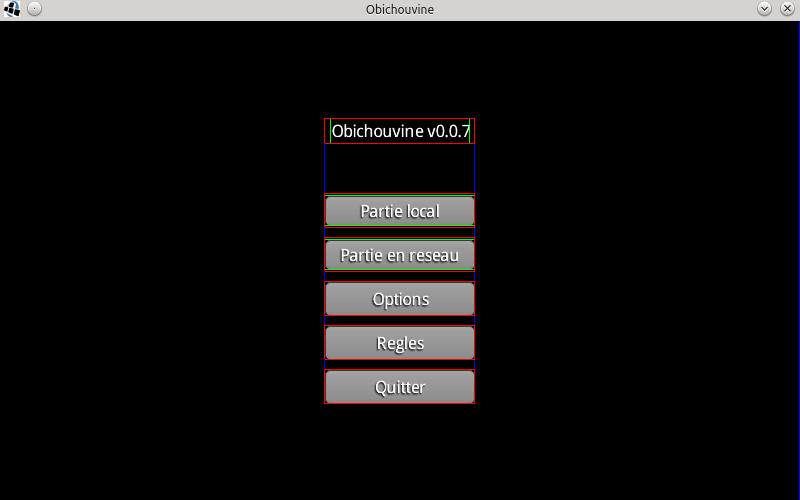
\includegraphics[width=9cm]{snapshot1.png}
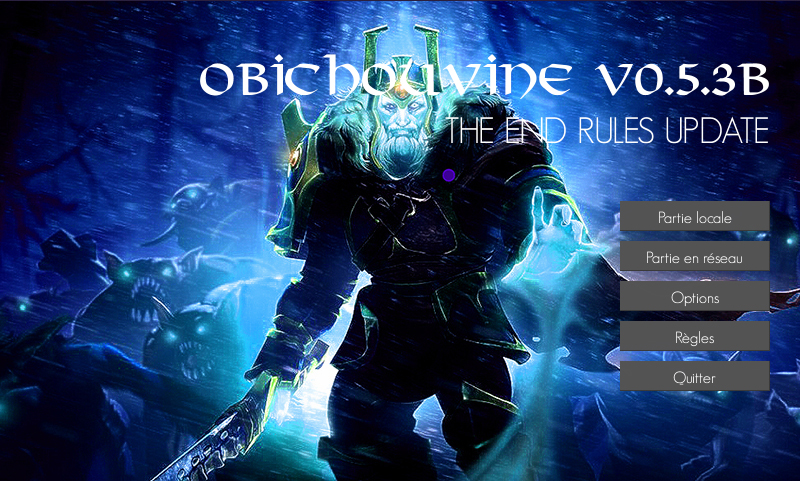
\includegraphics[width=9cm]{validDoc1.jpg}
\end{center}

\paragraph{}
Voici une comparaison entre la première et la dernière version du menu principal. Les améliorations ne sont que visuelle. De manière analogue, le menu "Options" a subi les mêmes mutations. A noté cependant, les cadres rouges et bleu autour des widgets ne font pas partie de l'interface. Ce sont des aides visuelles en mode "développeur" pour placer plus facilement les widgets sur les écrans. 

\paragraph{}
L'écran de lancement de partie locale a, par contre, été très lourdement modifié, comme en témoigne cette image :

\begin{center}
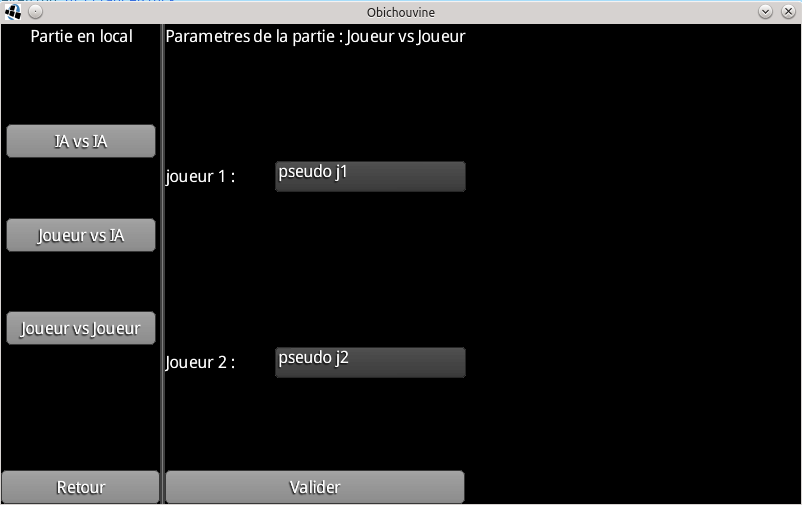
\includegraphics[width=7cm]{snapshot4.png}
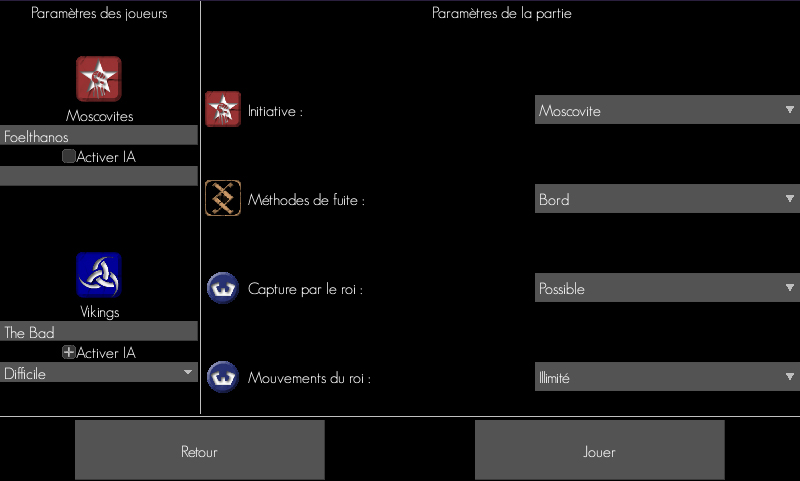
\includegraphics[width=7cm]{validDoc2.jpg}
\end{center}
\paragraph{}
Ces modifications ont été inspirés par les différentes audits ainsi que par les rencontres avec notre tuteur.
\paragraph{}
L'écran de jeu a également fortement évolué :

\begin{center}
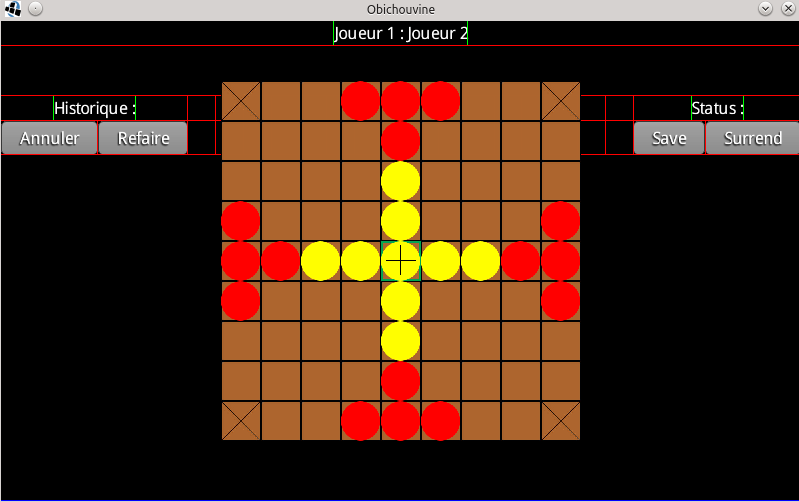
\includegraphics[width=10cm]{snapshot5.png}
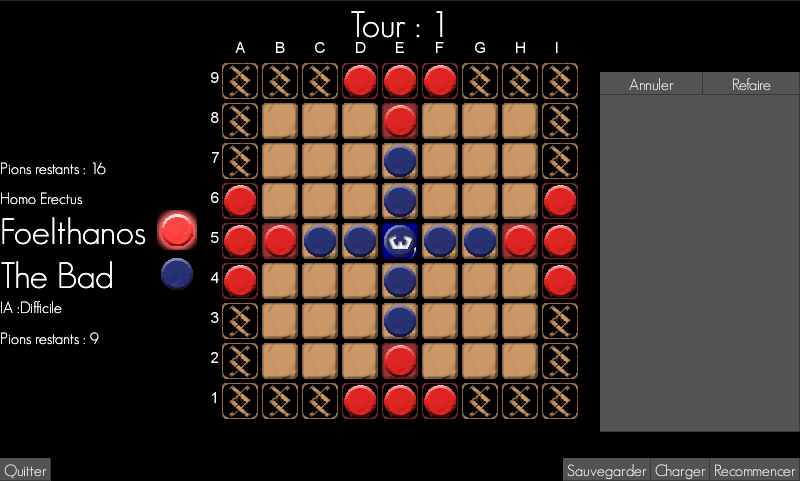
\includegraphics[width=10cm]{validDoc3.jpg}
\end{center}

\paragraph{}
Pour cet écran, ce n'est pas seulement des modifications visuelle mais surtout des modifications de confort de jeu. Surbrillance, changement de couleur, affichage des informations utiles, etc.
\paragraph{}
Un autre écran ayant subi de profonds changements est l'écran de règles :

\begin{center}
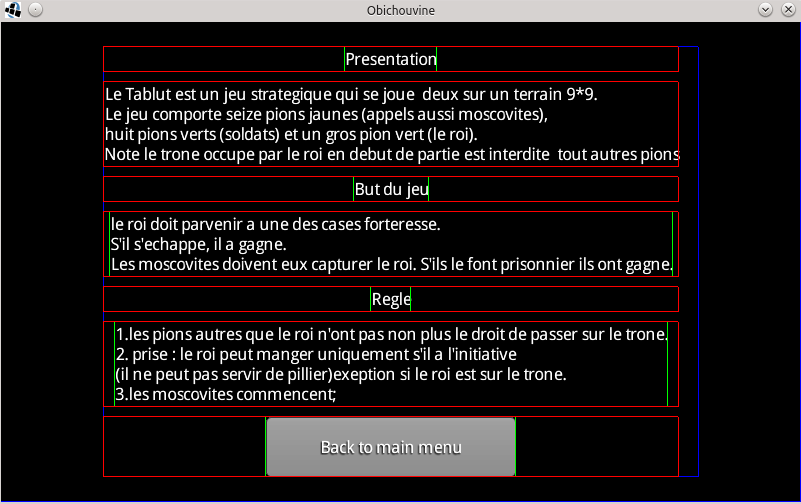
\includegraphics[width=10cm]{snapshot8.png}
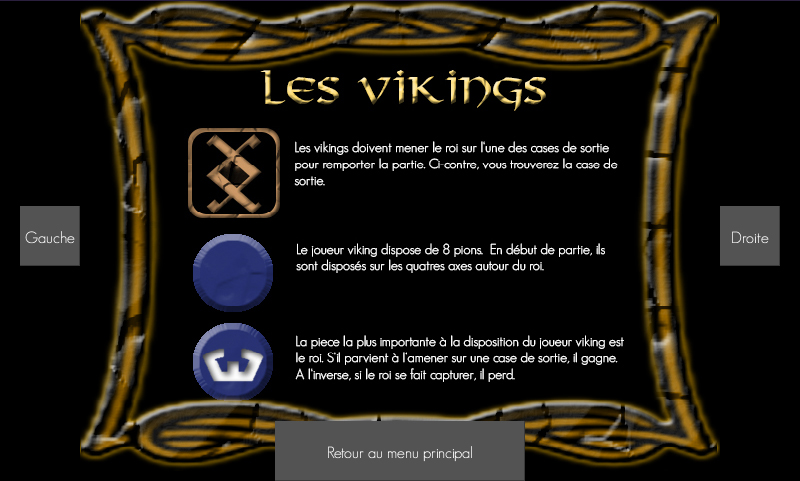
\includegraphics[width=10cm]{validDoc4.jpg}
\end{center}
\paragraph{}
La dernière version est directement inspiré des jeux flash en ligne et des jeux sur plate-forme mobile. En effet, ce genre de jeu dispose d'une explication des règles très visuelle permettant de faire un lien avec l'écran de jeu.

\section{Validation interne}
\paragraph{}
La validation interne a pour objectif de vérifier le bon fonctionnement technique de l'interface.

\subsection{Procédure}
\paragraph{}
La procédure est très simple pour les widgets au comportement simple (boutons, label, ...). Une fois le widget intégré, on lance l'application et on teste le widget. Si le comportement effectué par le widget est celui attendu, c'est validé.
\paragraph{}
Par contre, pour les widgets complexes, il peut y avoir plusieurs paramètres différents possibles pour une plage de résultat très varié. La procédure est donc plus stricte dans ces cas. Ces widgets complexes sont bien souvent. Voici la liste des widgets complexes utilisé pour ce programme :
\begin{itemize}
\item OptionPane
\item PlayerSelection
\item GameStatusWidget
\item HistoryWidget
\end{itemize}
\paragraph{}
Pour les valider, des jeux de tests sont mis en place. Toutes les possibilités doivent être couvertes.

\subsection{Bilan}
\subsubsection{OptionPane}
\paragraph{}
Le widget OptionPane est une interface permettant à l'utilisateur de générer un ensemble de paramètres. Ces paramètres modélisent les différentes variantes du jeu. Le widget récupère le Skin en entrée de manière à uniformiser l'apparence des widgets utilisés dans cette classe. L'OptionPane possède deux méthodes : printCommonContent() et generateParameter().
\paragraph{}
Le premier ne reçoit aucun paramètre et ne retourne rien, mais affiche les différents widgets que composent l'OptionPane. Pour vérifier le bon fonctionnement de cette méthode, on vérifie visuellement l'affichage de tous les widgets prévus. C'est le cas.
\paragraph{} 
L'un de ces widgets possèdent des écouteurs. Il faut donc également vérifier le bon fonctionnement du comportement voulu. Le widget en question est un menu déroulant. Il doit modifier l’icône correspondant à sa ligne du tableau. La vérification est encore une fois visuelle. Cela est validé.
\paragraph{}
La méthode generateParameter() est censé récupérer les données des widgets affichés et les formater pour permettre l'utilisation en cours de jeu. Il doit donc renvoyer un Parameter (classe créer dans ce but composé d'énumérations). 
\paragraph{}
La vérification se fait via l'entrée de chaque combinaison de données possibles et la vérification de l'exactitude de la sortie. Chaque combinaison a renvoyé le bon résultat. 

\subsubsection{PlayerSelection}
\paragraph{}
Le widget PlayerSelection est une interface permettant de générer une instance de données représentant un joueur, qu'il soit humain ou non. De manière analogue à OptionPane, le widget récupère un Skin en entrée et possède deux méthodes, l'une pour afficher les widgets l'autre pour formater la réponse globale de l'instance de PlayerSelection.
\paragraph{}
La vérification suit donc exactement le même protocole. Tous les widgets prévues sont affichés. De même pour l'écouteur du widget de case à cocher. Le comportement attendu est de rafraîchir le modèle de l'instance de PlayerSelection. Une subtilité existe tout de même. Lorsque la checkbox est cochée, il faut impérativement que la liste déroulante du widget soit désactivé. La vérification confirme ce fait.
\paragraph{}
A l'instar de l'OptionPane, la méthode de récupération est vérifiée par un simple affichage dans la console. Le widget PlayerSelection est également validé.

\subsubsection{GameStatusWidget}
\paragraph{}
Ce widget agit légèrement différemment des autres widgets. Au lieu d'être composé de widgets disposant d’écouteur permettant la modification de son modèle, il reçoit des événements extérieurs. La validation de l'affichage est donc semblable mais pas celle des écouteurs car ils n'existent pas. Certaines méthodes sont appelées par la classe appelante, ce qui induit une modification de certains de ses attributs et rafraîchit les widgets concernés.
\paragraph{}
Heureusement pour les tests, il n'y a qu'une seule méthode à valider, switchTurn(). Elle doit inverser la valeur d'une énumération (soit moscovites, soit vikings). Le widget est validé.

\subsubsection{HistoryWidget}

\paragraph{}

\section{Validation externe}
\paragraph{}
La validation externe a pour objectif d'améliorer l’expérience de l'utilisateur en recueillant les idées et critiques de personnes externes au projet.

\subsection{Panel d'utilisateurs}
\paragraph{}
La validation dite "externe" est divisé en deux catégories : la validation durant le développement et la validation en bêta-test. 
\paragraph{}
Durant le développement, quatres personnes ont permis les améliorations successives de l'ergonomie de l'interface : le responsable de l'audit IHM, notre tuteur ainsi que deux personnes extérieures au projet. Cette validation est nécessaire pour corriger rapidement les erreurs de conception trop graves très vite durant le développement.
\paragraph{}
La bêta-test a été effectué le week-end du samedi 7 juin à 10h au dimanche 8 juin à 18h. 15 personnes ont participé à ce week-end de bêta-test. Voici les principales informations sur l'échantillon :

\begin{center}
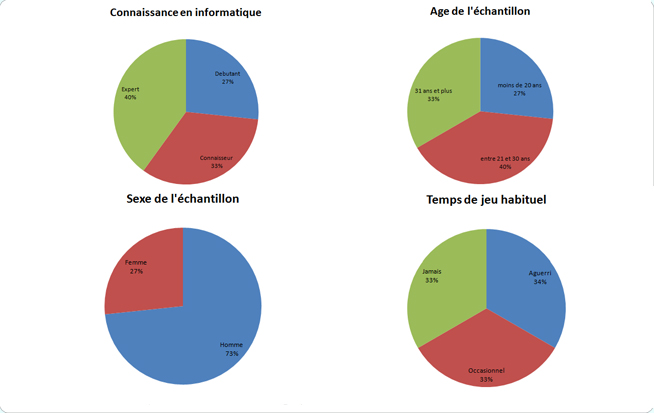
\includegraphics[width=15cm]{echantillon.jpg}
\end{center}

\paragraph{}
Parmi les "experts" en informatique, une personne est développeur professionnel dans le domaine du jeu vidéo tandis qu'une autre personne étudie actuellement dans ce sens. Cet échantillon est relativement équilibré et permet de s'assurer d'une ergonomie efficace pour le public le plus large possible.

\paragraph{}
Ce panel varié nous permettra de recueillir des informations variées. Nous pourrons ainsi utiliser ces informations afin d'optimiser l'ergonomie du jeu pour le public le plus large possible.

\subsection{Déroulement de l'évaluation}
\paragraph{}
Durant le développement, l’évaluation est surtout faite via des retours directs. Lors de discussions sur Skype ou via des audits/rencontres avec le tuteurs. Lors des audits, nous faisons tourner le jeu et le professeur émet ses interrogations et avis durant la présentation. 
\paragraph{}
En ce qui concerne la bêta-test, nous envoyons la première version bêta par mail avec des directives et plusieurs documents. Les documents en question sont un sondage sur l'ergonomie du jeu et un tableau de rapport de bogues. Nous demandons à tous les participants d'être le plus honnêtes possibles lors du remplissage de ces documents.
\paragraph{}
Le sondage est principalement orienté sur la qualité de l'interface mais quelques questions ont été réservés pour l'intelligence artificielle. 

\subsection{Bilan}

\begin{center}
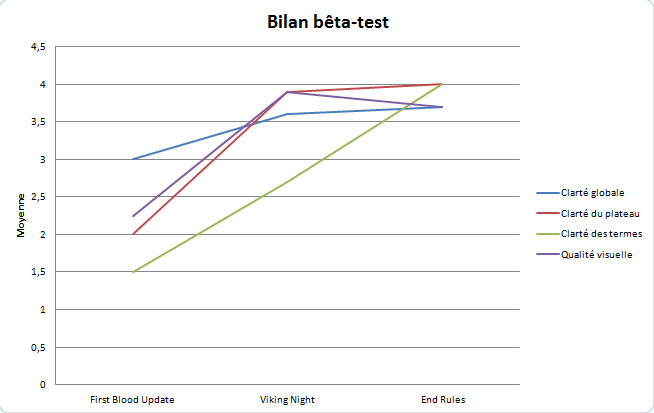
\includegraphics[width=15cm]{resBeta.jpg}
\end{center}

\paragraph{}
Ce graphique rassemble les moyennes des notes attribuées par les testeurs pour chacun des principaux patchs de la phase de bêta-test. 
\paragraph{}
On remarque les faibles notes pour le premier patch, surtout pour la clarté des termes. L’échantillon était de seulement quatres personnes, ce n'est donc pas très représentatif, mais cela traduisait un grand manque d'explication des règles du jeu. On remarque également des notes mauvais en ce qui concerne la clarté des informations de l’écran de jeu ainsi que de la qualité visuelle du logiciel.
\paragraph{}}
La mise à jour suivante, nommée "Viking Night Update", à grandement améliorer la qualité visuelle ainsi que la clarté du plateau de jeu via une mise à jour de tous les sprites du jeu. De plus, la surbrillance a été amélioré. Un meilleur retour sur les actions de l'IA ont également été ajouté à travers une image indiquant que l'IA travaille. Ces efforts ont été récompensé par une amélioration nettes des notes. Cependant, cela restait très faible en ce qui concerne la clarté des explications. 
\paragraph{}
La dernière mise à jour du week-end a donc tenter d'améliorer l'explication des règles du jeu à travers un menu de règles plus précis et plus propre. L'utilisation des sprites du plateau de jeu permet un rappel visuel. Ce nouveau menu a été récompensé par une augmentation significative des notes en ce qui concerne l'explication des règles du jeu. 
\paragraph{}
En conclusion, la bêta-test a été concluante pour trouver les failles de l'interface, mais il reste encore du chemin.
\end{document}
